\documentclass{beamer}

\usepackage{graphicx}
\usepackage[utf8]{inputenc}

\title{GCM; The illegal attack}
\author{Mathias Hall-Andersen (rot256)}
\institute{Pwnies @ Copenhagen University}
\date{2017}

\begin{document}

\frame{\titlepage}

\begin{frame}
\frametitle{Authenticated encryption}
Why
\end{frame}

\begin{frame}
\frametitle{Galois Counter Mode}
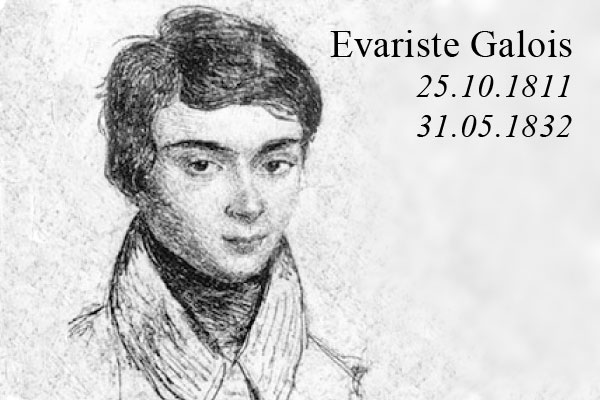
\includegraphics[width=\textwidth]{evariste_galois}
\end{frame}

\begin{frame}
\frametitle{Some basic algebra}
\end{frame}

\begin{frame}
\frametitle{Galois Counter Mode (continued)}
\end{frame}

\begin{frame}
\frametitle{Sage}
\end{frame}

\begin{frame}
\frametitle{Nonce reuse attack}
Theorists \& mathematicians care about proofs. \\
Hackers care about assumptions.
\end{frame}

\begin{frame}
\frametitle{Work session}
\end{frame}

\begin{frame}
\frametitle{Truncated nonce attack}
\end{frame}

\end{document}
